\section{Durchführung}
\label{sec:Durchführung}

\subsection{Versuchsaufbau}
Der Versuchsaufbau ist in Abb. \ref{fig:aufbau} zu sehen.
Das Licht der Rubidium-Spektrallampe trifft zunächst auf eine Sammellinse. Anschließend geht es durch einen Interferenzfilter (D$_1-$Filter), der nur Licht mit einer Wellenlänge von $\lambda = \SI{794.8}{\nano\meter}$ durchlässt. Der darauffolgende Polarisationsfilter und die $\lambda / 4-$Platte bewirken, dass das austretende Licht rechtszirkular polarisiert ist. Dieses Licht trifft auf die von drei Helmholtz-Spulenpaaren umgebene Dampfzelle. Das transmittierte Licht wird mithilfe einer Sammellinse auf einen Lichtdetektor fokussiert, welcher an einem Oszilloskop angeschlossen ist. \cite{V21}

\begin{figure}
    \centering
    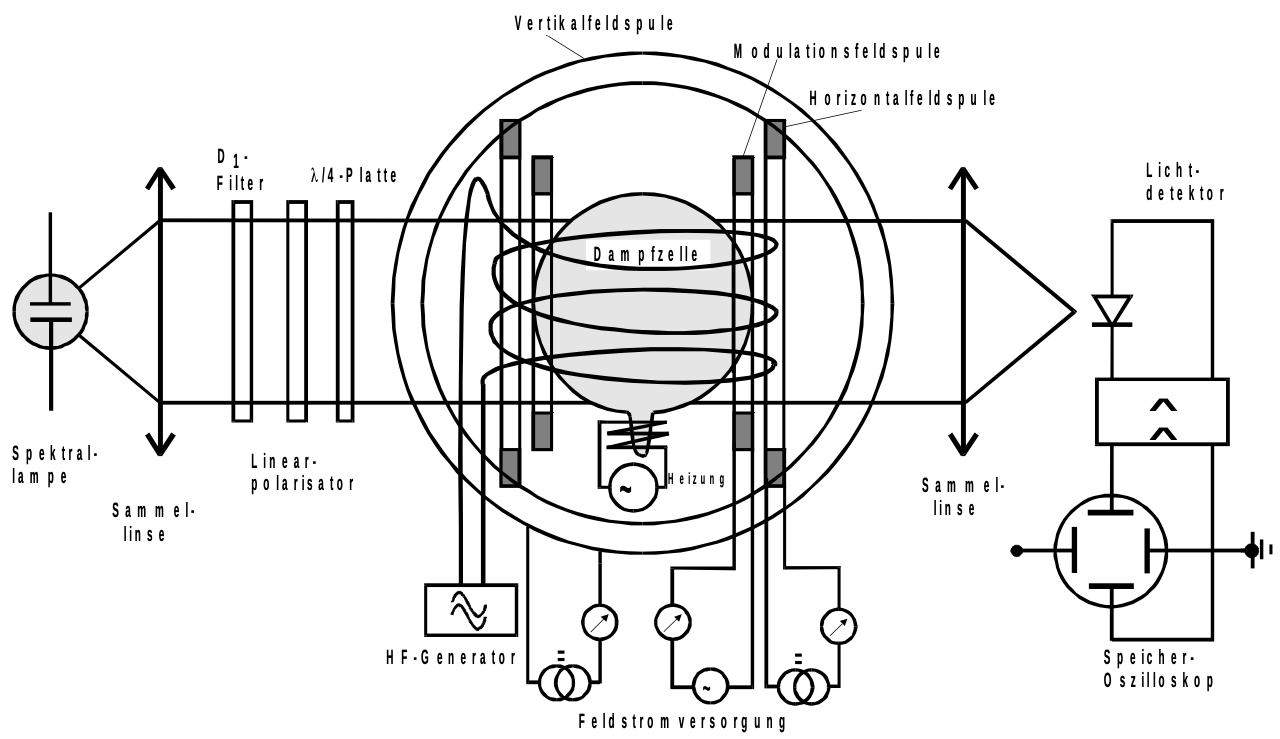
\includegraphics[width=15cm]{fotos/aufbau.png}
    \caption{Der Aufbau der Messapparatur. \cite{V21}}
    \label{fig:aufbau}
\end{figure}

Die Eigenschaften der Spulen sind in Tab. \ref{tab:spule} aufgelistet. 
Alle drei Spulen sind Helmholtzspulen-Paare. Für sie gilt, dass die Magnetfeldstärke 
\begin{equation}
    B = \mu_0 \cdot \frac{8 \cdot I \cdot N}{\sqrt{125} R}
    \label{eq:B}
\end{equation}
beträgt mit der Stromstärke $I$, der Windungszahl $N$ und dem Radius $R$. 

\begin{table}\caption{Die Werte der Horizontal-, Sweep- und Vertikalspule. Alle drei sind Helmholtzspulen-Paare.}
    \label{tab:spule}
    \centering
    \sisetup{round-mode = places, round-precision=1, round-integer-to-decimal=true}
    \begin{tabular}{c | S[] S[] S[]} 
    \toprule
    {Spule} & {$R / \si{\centi\metre}$} & {$N$} & {Verstärkung} \\
    \midrule
    Horizontal & 15.79 & 154 & 0.3 \\
    Sweep & 16.39 & 11 & 0.1 \\ 
    Vertikal & 11.735 & 20 & 0.1 \\ 
    \bottomrule
\end{tabular}\end{table}


\subsection{Justierung}
Der Ofen, der die Dampfzelle heizt, wird eine halbe Stunde vor Beginn eingeschaltet.
Zunächst wird der Strahlengang so justiert, dass die Intensität maximal ist. Diese wird am Lichtdetektor gemessen.
%Dazu ist der "Gain" überall $\num{1}$ und die Zeitkonstante beträgt $\SI{100}{\milli\second}$.
Anschließend werden die beiden Linsen eingesetzt und mithilfe der Signalstärke am Galvanometer justiert.
Nachdem weitere optische Elemente eingesetzt sind, wird der ganze Aufbau mit einer schwarzen Decke abgedeckt. \cite{V21}

Vor der Messung muss das Erdmagnetfeld kompensiert werden.
Dazu wird durch einen Stromfluss durch die Sweep-Spule (Modulationsfeldspule) die horizontale Magnetfeldkomponente auf Null reguliert. Anschließend wird mithilfe der Vertikalfeldspule ein schmaler Peak eingestellt, um die Vertikalkomponente des Erdmagnetfeldes zu kompensieren. Die Messapparatur wird so ausgerichtet, dass der Lichtstrahl in Nord-Süd-Richtung verläuft. \cite{V21}

\subsection{Messung der Resonanzstellen}

Die Frequenz an den RF-Spulen wird zwischen $\SI{100}{\kilo\hertz}$ und $\SI{1}{\mega\hertz}$ in $\SI{100}{\kilo\hertz}$ Schritten variiert. Dabei wird die Stärke des gesamten Horizontalfeldes in Abhängigkeit von der Resonanzfrequenz für beide Rb-Isotope gemessen. Die Resonanzen für beide Isotope sollen sichtbar gemacht werden. Bei Frequenzen höher als $\SI{200}{\kilo\hertz}$ wird zusätzlich ein horizontales Feld angelegt.

Es wird ein Foto eines typischen Signalbildes bei $\SI{100}{\kilo\hertz}$ gemacht.